\documentclass[a4paper,12pt, oneside]{article}   	
	
\usepackage[utf8x]{inputenc}
\usepackage[english,greek]{babel}
\usepackage[margin=1.2in]{geometry}
\usepackage[parfill]{parskip}    	
\usepackage{microtype}
\usepackage{graphicx}
\usepackage{wrapfig}
\usepackage{enumitem}
\usepackage{fancyhdr}
\usepackage{amsmath,amsfonts,amssymb}
\usepackage{cite}
\usepackage{subcaption}
\usepackage{float}
\usepackage{titlesec}
\usepackage{index}
\makeindex

%SetFonts
\usepackage{lmodern}
%SetFonts

\usepackage[unicode=true]{hyperref}

\addto\captionsgreek{ \renewcommand{\listfigurename}{Διαγράμματα \textlatin{UML}}}

\pagestyle{fancy}
\fancyhf{}
\renewcommand{\headrulewidth}{0pt}
\fancyhead[RE]{}
\fancyhead[RO]{}
\fancyfoot[RE, RO]{\thepage}


\titleformat{\section}
  {\normalfont\Large\bfseries}{\thesection}{1em}{}[{\titlerule[0.8pt]}]

\begin{document}
\makeatletter
\renewcommand\paragraph{\@startsection{paragraph}{4}{\z@}%
            {-2.5ex\@plus -1ex \@minus -.25ex}%
            {1.25ex \@plus .25ex}%
            {\normalfont\normalsize\bfseries}}
\makeatother
\setcounter{secnumdepth}{4} % how many sectioning levels to assign numbers to
\setcounter{tocdepth}{4}    % how many sectioning levels to show in ToC



\begin{titlepage}
\begin{center}


\includegraphics[width=0.20\textwidth]{./img/NTUAlogo.jpg}~\\[0.1cm]
\textsc{ ΕΘΝΙΚΟ ΜΕΤΣΟΒΙΟ ΠΟΛΥΤΕΧΝΕΙΟ}\\[0.2cm]  
\textsc{ ΣΧΟΛΗ ΗΛΕΚΤΡΟΛΟΓΩΝ ΜΗΧΑΝΙΚΩΝ ΚΑΙ ΜΗΧΑΝΙΚΩΝ ΥΠΟΛΟΓΙΣΤΩΝ}\\[3cm] 


\textbf{\LARGE Έγγραφο απαιτήσεων λογισμικού\textlatin{ (SRS)}}\\[0.01cm]
\text{Σύμφωνα με το πρότυπο \textlatin{ISO/IEC/IEEE 29148:2011}}\\[2cm]


% Author and supervisor 
\textbf{Ομάδα:  \textlatin{WeAreBack}}\\
	Σταύρος Σταύρου \\
	Λένος Τσοκκής \\ 
	Κωνσταντίνα Φουντουραδάκη
\vfill

\end{center} 
\end{titlepage}

\thispagestyle{empty}
\pagenumbering{gobble}% Remove page numbers (and reset to 1)
\newpage

\thispagestyle{empty}
\pagenumbering{arabic}
\setcounter{page}{2}
\tableofcontents
\clearpage
\listoffigures
\newpage


\section{Εισαγωγή}
\subsection{Σκοπός του λογισμικού}
O σκοπός της ομάδας \textlatin{WeAreBack} είναι η υλοποίηση μιας πλατφόρμας παρατήρησης κατανάλωσης/παραγωγής ενέργειας στην οποία μπορεί οποιοσδήποτε να έχει ελεύθερη πρόσβαση. Απευθύνεται κυρίως σε εταιρίες παραγωγής ή παροχής ενέργειας, σε Υπουργεία Ενέργειας εντός Ευρωπαϊκής Ένωσης, στον απλό πολίτη και στους δημοσιογράφους. Η πλατφόρμα θα προσφέρει στους χρήστες υπηρεσίες όπως πρόσβαση σε ένα μεγάλο σύνολο δεδομένων παραγωγής και κατανάλωσης ενέργειας, προβλέψη της μελλοντκής κατανάλωσης ανά τύπο ενέγειας και σύγκριση της προβλεπόμενης με την πραγματική κατανάλωση. Επιπλέον, πρωτεύοντες στόχοι είναι η ευχρηστία πλατφόρμας, η τεκμηρίωση και η συντήρηση του κώδικα. Τέλος, αφορμή για την υλοποίηση του συστήματος συνιστούν η αναγκαιότητα της ενέργειας και η διαχείριση της, λόγοι για τους οποίους η πλατφόρμα θα μπορεί να διαδοθεί ευρέως.


\subsection{Διεπαφές \textlatin{(interfaces)}}
\subsubsection{Διεπαφές με εξωτερικά συστήματα και εφαρμογές λογισμικού}

\begin{figure}[h]
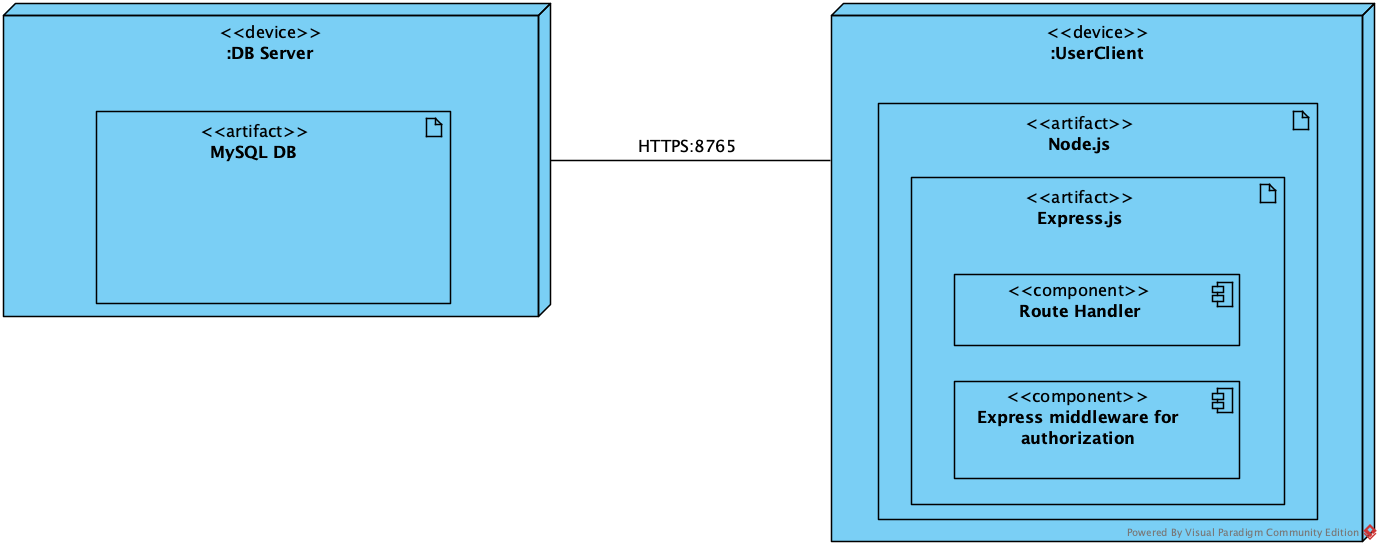
\includegraphics[width=1\textwidth]{./UML/Deployment_Diagram.png}
\caption{\textlatin{Deployment diagram}}
\centering
\end{figure}

\clearpage

\subsubsection{Διεπαφές με το χρήστη}
\begin{figure}[h]
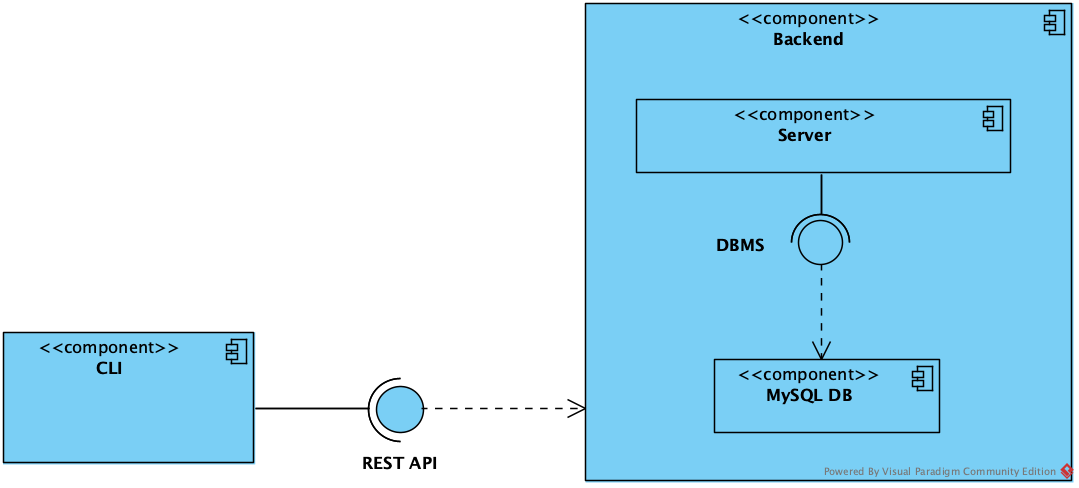
\includegraphics[width=1\textwidth]{./UML/Component_Diagram.png}
\caption{\textlatin{Component diagram}}
\centering
\end{figure}


\section{Αναφορές}
\begingroup
\renewcommand{\section}[2]{}
\begin{thebibliography} {books}
\latintext
\bibitem{ISO2011} ISO/IEC 29148:2011 (IEEE Std 29148-2011), Systems and software engineering - Life cycle processes - Requirements engineering
\end{thebibliography}
\endgroup

\subsection*{Πηγές Πληροφοριών}
\latintext
\href{https://www.visual-paradigm.com/guide/}{https://www.visual-paradigm.com/guide/} \\
\href{https://swagger.io/specification/}{https://swagger.io/specification/}\\
\href{https://medium.com/@mihaigeorge.c/web-rest-api-benchmark-on-a-real-life-application-ebb743a5d7a3}{https://medium.com/@mihaigeorge.c/web-rest-api-benchmark-on-a-real-life-application-ebb743a5d7a3}\\
\href{https://medium.com/hackernoon/back-end-performance-those-metrics-we-care-about-ade678e87969}{https://medium.com/hackernoon/back-end-performance-those-metrics-we-care-about-ade678e87969}
\newpage
\greektext

\section{Προδιαγραφές απαιτήσεων λογισμικού} 
\subsection{Περιπτώσεις χρήσης}
\subsubsection{ΠΕΡΙΠΤΩΣΗ ΧΡΗΣΗΣ 1: Ανάκτηση δεδομένων από Απλό Χρήστη}
\paragraph{Χρήστες (ρόλοι) που εμπλέκονται}
Στη συγκεκριμένη περίπτωση εμπλέκεται μόνο ο Απλός Χρήστης, ο οποίος συνδέεται στην πλατφόρμα και ανακτά δεδομένα ενέργειας από τη βάση δεδομένων.
 
\paragraph{Προϋποθέσεις εκτέλεσης}
Προϋποθέσεις πρόσβασης του Χρήστη στα δεδομένα που επιθυμεί, είναι η σύνδεση του στην πλατφόρμα, η διαπίστευση του \textlatin{(user access token)}, να έχει επαρκή \textlatin{quota} και να έχει διατυπώσει σωστά την εντολή στο \textlatin{CLI}. Μια επιπλέον προϋπόθεση είναι η πλήρη συνδεσιμότητα του χρήστη με τη βάση δεδομένων, που μπορεί να ελεγχθεί μέσω  του \textlatin{endpoint HealthCheck}.

\paragraph{Περιβάλλον εκτέλεσης}
Το περιβάλλον εκτέλεσης της περίπτωσης χρήσης είναι το \textlatin{CLI}, το οποίο είναι διαθέσιμο μόνο από την κονσόλα \textlatin{(command line, ssh)} του συστήματος που φιλοξενεί την εφαρμογή.

\paragraph{Δεδομένα εισόδου}
Ως δεδομένα εισόδου θεωρούμε το  \textlatin{username} και  \textlatin{password} που εισάγει ο χρήστης προκειμένου να συνδεθεί στην πλατφόρμα, καθώς και η εντολή που δίνει στο  \textlatin{CLI}. \\
Οι συνθήκες εγκυρότητας για τα παραπάνω είναι η ταυτοποίηση του χρήστη και σωστή χρήση των παραμέτρων που  δίνονται σε μία κλήση (διαφορετικά  το  \textlatin{API} επιστρέφει  \textlatin{HTTP Status Code 400, "Bad Request").}
Οι συνθήκες εγκυρότητας εξόδου είναι η ύπαρξη των δεδομένων που ζήτησε ο χρήστης (διαφορετικά  το  \textlatin{API} επιστρέφει  \textlatin{HTTP Status Code 403, "No data").}

\paragraph{Αλληλουχία ενεργειών - επιθυμητή συμπεριφορά}
Αλληλουχία ενεργειών: \\
\begin{enumerate}
	\item Πρόσβαση στο \textlatin{CLI}
	\item Εντολή εισόδου συνοδευόμενη από τα στοιχεία εισόδου
	\item Επιστρέφεται το token στον χρήστη
	\item Εντολή για προσπέλαση δεδομένων
	\item Επιστρέφονται στον χρήστη τα ζητούμενα δεδομένα είτε με μορφή \textlatin{JSON} \\είτε \textlatin{csv}
\end{enumerate} 

\begin{figure}[h]
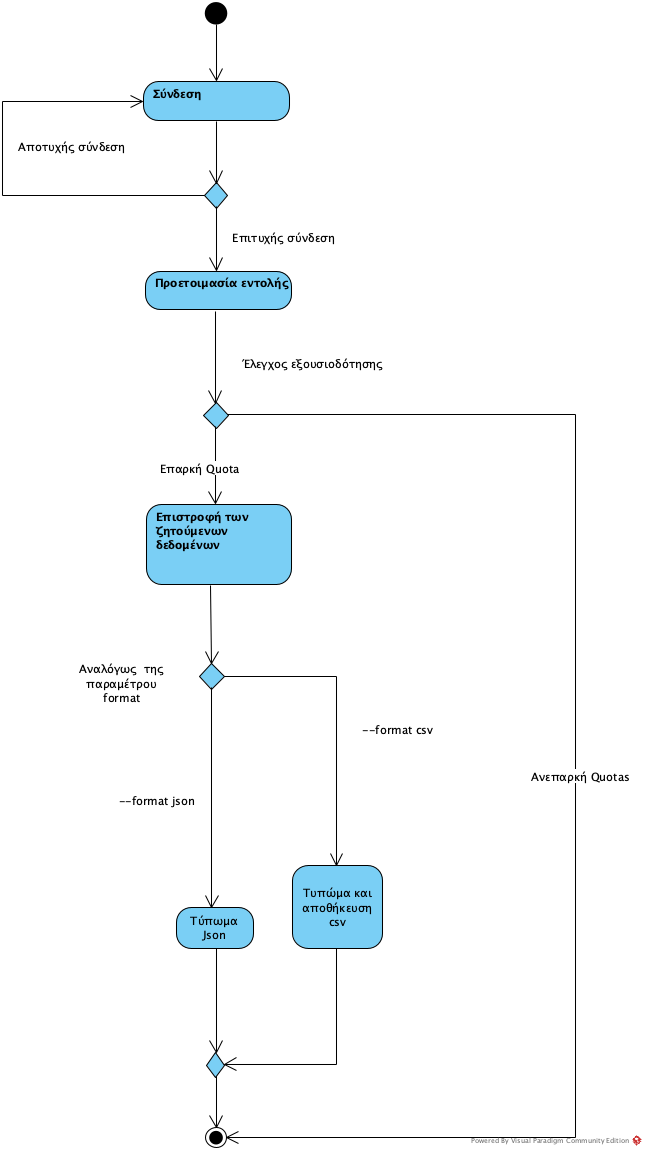
\includegraphics[width=0.8\textwidth]{./UML/Activity_Diagram_User.png}
\caption{\textlatin{Activity diagram} Απλού Χρήστη}
\centering
\end{figure}
\clearpage


\begin{figure}[h]
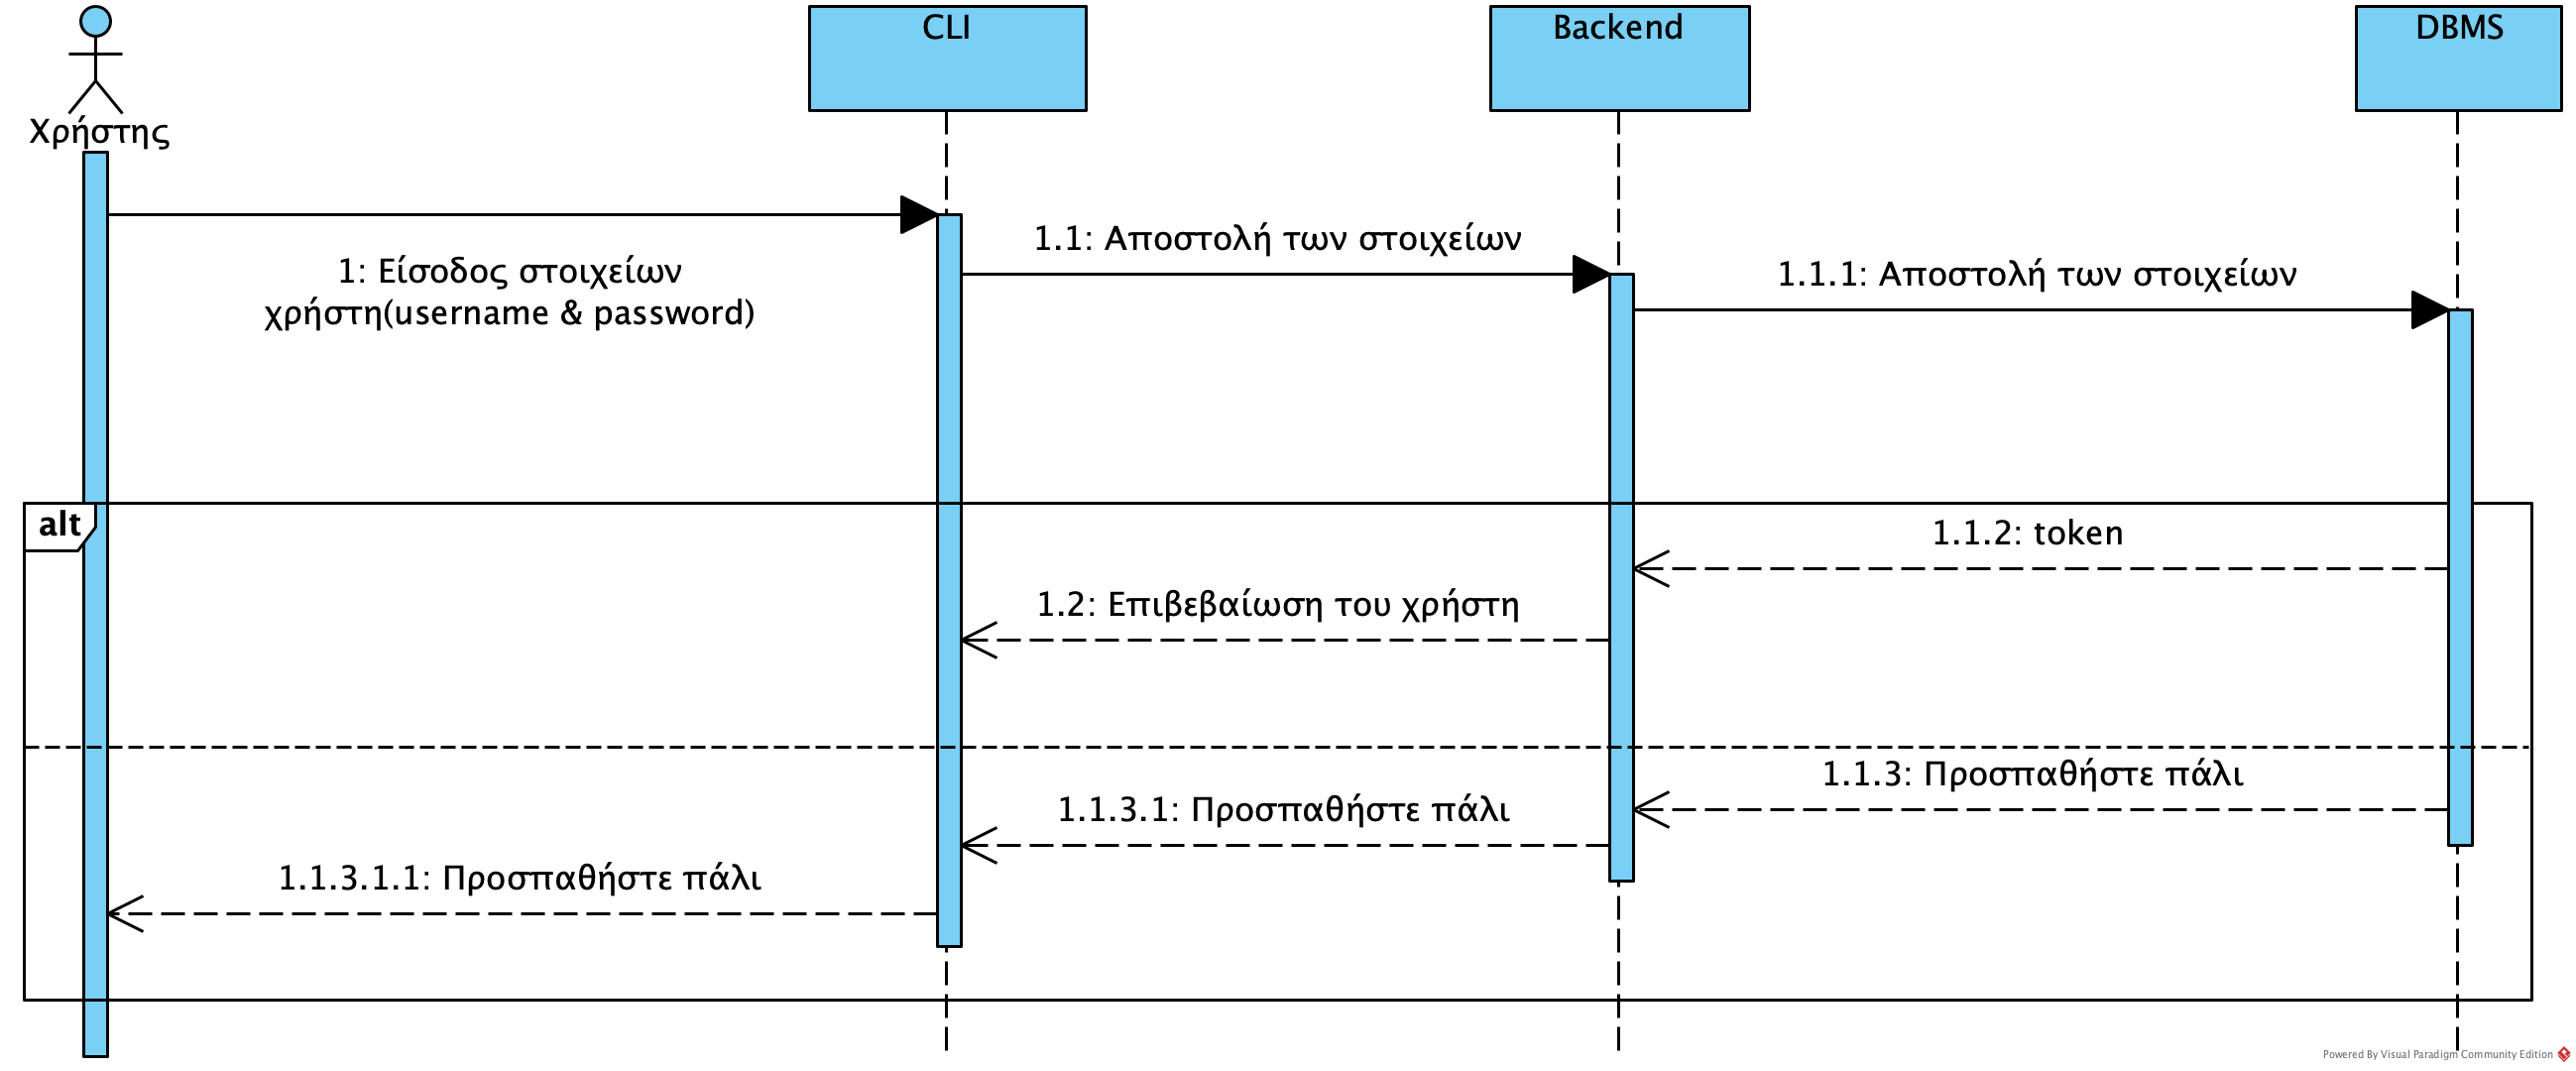
\includegraphics[width=1\textwidth]{./UML/Sequence_Diagram_User_Login.png}
\caption{\textlatin{Sequence diagram} εισόδου Απλού Χρήστη}
\centering
\end{figure}

Αλληλουχία ενεργειών για προσπέλαση δεδομένων: \\
\begin{enumerate}
	\item Εντολή για προσπέλαση δεδομένων
	\item Ελέγχεται αν η μορφή της εντολής είναι έγκυρη
	\item Ελέγχεται αν ο χρήστης έχει διαθέσιμα \textlatin{quota}
	\item Ελέγχεται αν ο χρήστης είναι εξουσιοδοτημένος για αυτή την ενέργεια
	\item Επιστρέφονται στον χρήστη τα ζητούμενα δεδομένα είτε με μορφή \textlatin{JSON} \\είτε \textlatin{csv}, αν υπάρχουν και μειώνεται το \textlatin{quota}
\end{enumerate} 
\clearpage

\begin{figure}[h]
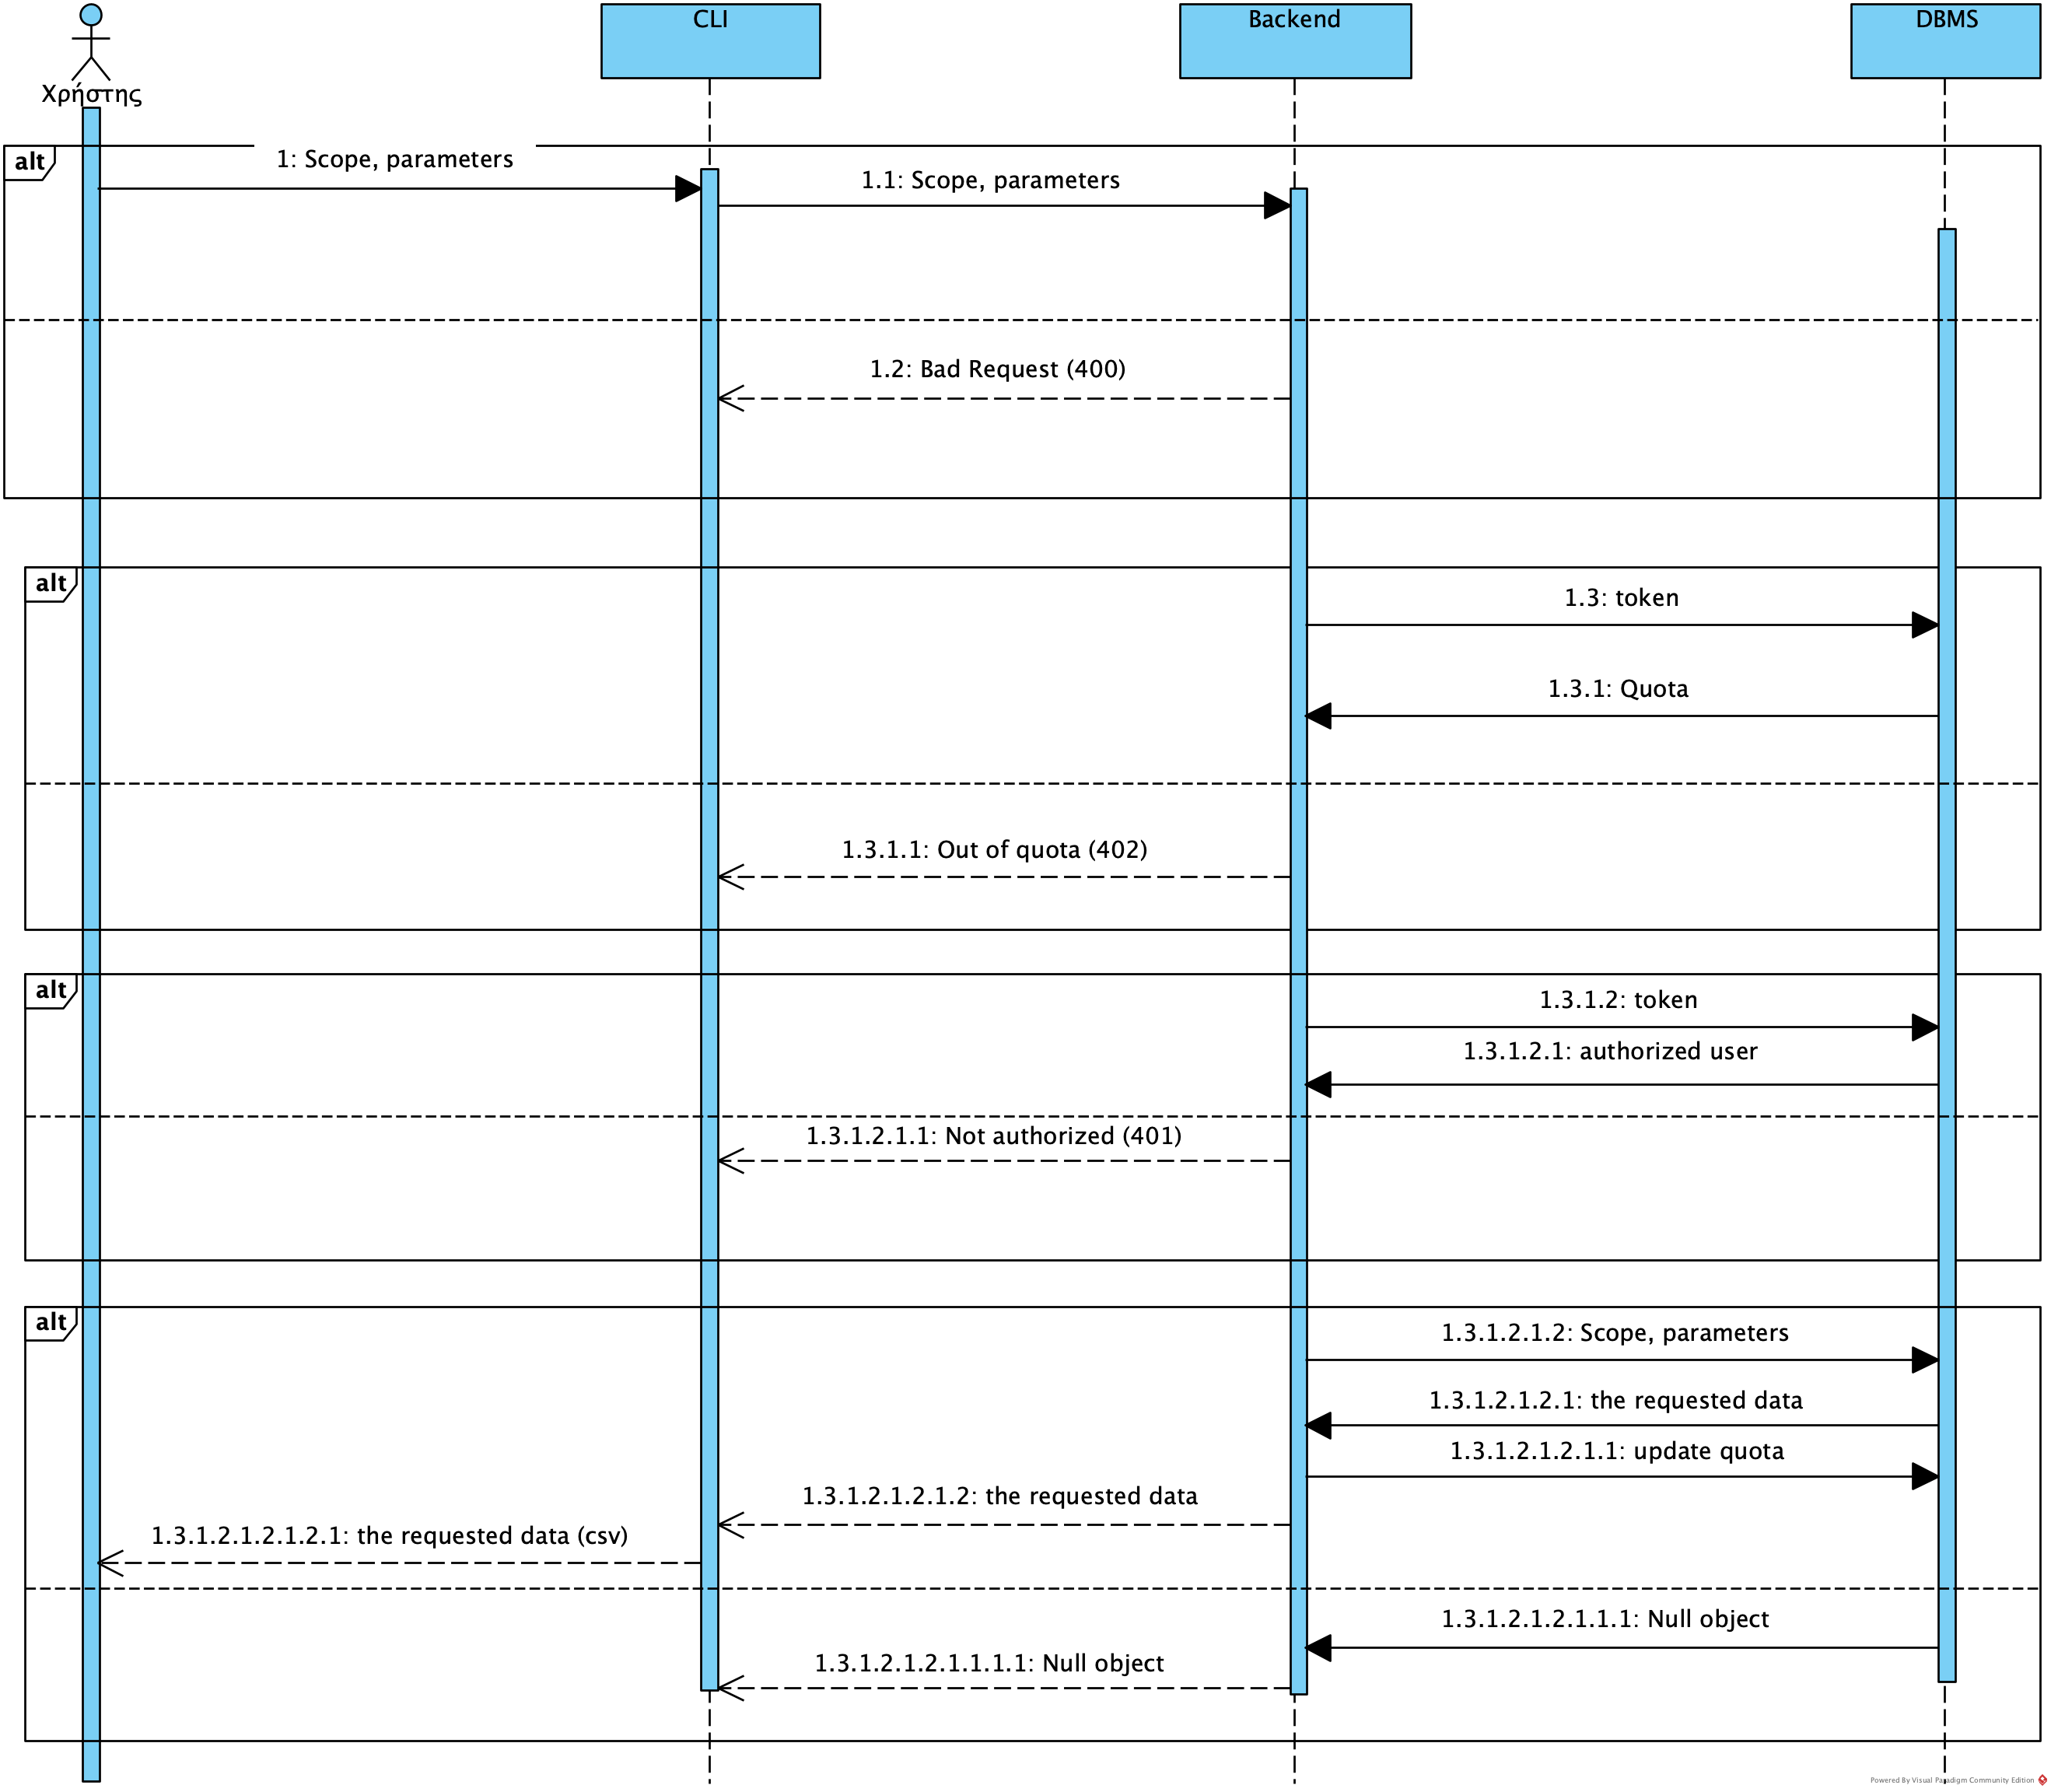
\includegraphics[width=1\textwidth]{./UML/Sequence_Diagram_User_get_data.png}
\caption{\textlatin{Sequence diagram} ανάκτησης δεδομένων από Απλό Χρήστη}
\centering
\end{figure}


\paragraph{Δεδομένα εξόδου}
Εάν η παράμετρος \textlatin{format} της εντολή στο \textlatin{CLI}, έχει οριστεί ως \textlatin{csv} τότε δημιουργείται έαν αρχείο \textlatin{.csv} που περιέχει τα δεδομένα που ζήτησε ο χρήστης.



\newpage
\subsubsection{ΠΕΡΙΠΤΩΣΗ ΧΡΗΣΗΣ 2: Εμφάνιση κατάστασης ενός χρήστη από τον Διαχειριστή}
\paragraph{Χρήστες (ρόλοι) που εμπλέκονται}
Στη συγκεκριμένη περίπτωση εμπλέκεται ο Διαχειριστής, ο οποίος συνδέεται στην πλατφόρμα και ο Χρήστης του οποίου τα στοιχεία κατάστασης θέλει να προσπελάσει ο Διαχειριστής από τη βάση δεδομένων.

\paragraph{Προϋποθέσεις εκτέλεσης}
Προϋποθέσεις πρόσβασης του Διαχειριστή στη βάση δεδομένων για να ανακτήση την κατάσταση κάποιου χρήστη, είναι η σύνδεση του στην πλατφόρμα, η διαπίστευση του ως διαχειριστή \textlatin{(user access token)} και να έχει διατυπώσει σωστά την εντολή στο \textlatin{CLI}. Μια επιπλέον προϋπόθεση είναι η πλήρη συνδεσιμότητα του χρήστη με τη βάση δεδομένων, που μπορεί να ελεγχθεί μέσω του \textlatin{endpoint HealthCheck}.

\paragraph{Περιβάλλον εκτέλεσης}
Το περιβάλλον εκτέλεσης της περίπτωσης χρήσης είναι το \textlatin{CLI}, το οποίο είναι διαθέσιμο μόνο από την κονσόλα \textlatin{(command line, ssh)} του συστήματος που φιλοξενεί την εφαρμογή.

\paragraph{Δεδομένα εισόδου}
Ως δεδομένα εισόδου θεωρούμε το  \textlatin{username} και  \textlatin{password} που εισάγει ο Διαχειριστής προκειμένου να συνδεθεί στην πλατφόρμα, καθώς και η εντολή που δίνει στο  \textlatin{CLI}. \\
Οι συνθήκες εγκυρότητας για τα παραπάνω είναι η ταυτοποίηση του ως Διαχειριστή και σωστή χρήση των παραμέτρων που δίνονται σε μία κλήση (διαφορετικά  το  \textlatin{API} επιστρέφει  \textlatin{HTTP Status Code 400, "Bad Request").}
Οι συνθήκες εγκυρότητας εξόδου είναι η ύπαρξη του χρήστη που αντιστοιχεί στο δοθέν \textlatin{username} (διαφορετικά  το  \textlatin{API} επιστρέφει  \textlatin{HTTP Status Code 403, "No data").}


\paragraph{Αλληλουχία ενεργειών - επιθυμητή συμπεριφορά}
Αλληλουχία ενεργειών: \\
\begin{enumerate}
	\item Πρόσβαση στο \textlatin{CLI}
	\item Εντολή εισόδου συνοδευόμενη από τα στοιχεία εισόδου
	\item Επιστρέφεται το token στον χρήστη
	\item Εντολή για προσπέλαση των στοιχείων κάποιου χρήστη
	\item Επιστρέφονται στον διαχειριστή τα ζητούμενα δεδομένα
\end{enumerate} 

\begin{figure}[h]
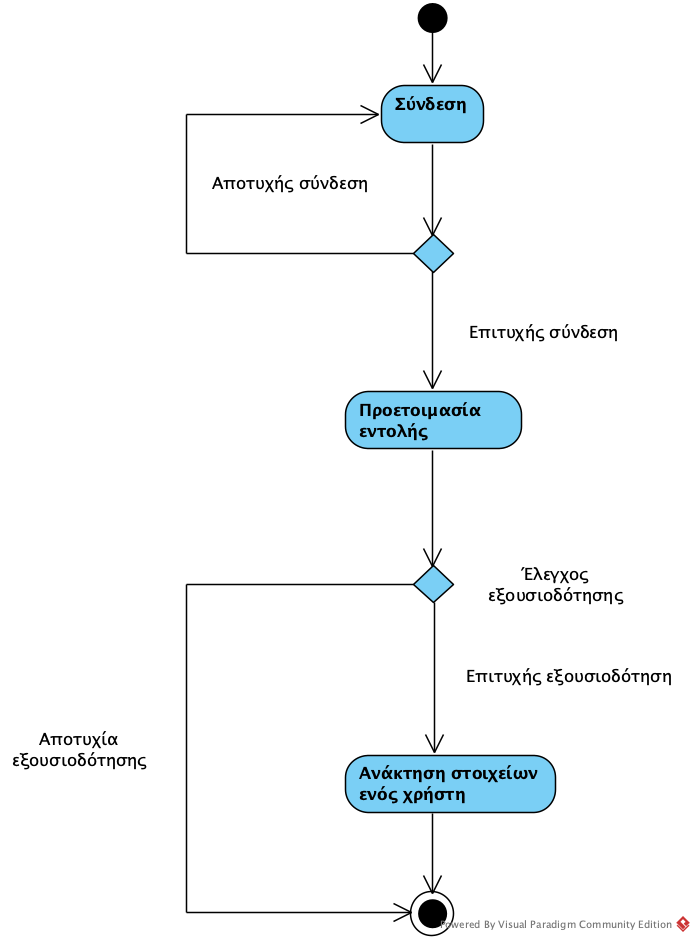
\includegraphics[width=0.8\textwidth]{./UML/Activity_Diagram_Admin_fetch_userstatus.png}
\caption{\textlatin{Activity diagram} Διαχειριστή, όπου ζητάει πληροφορίες για κάποιο χρήστη}
\centering
\end{figure}
\clearpage


Αλληλουχία ενεργειών για προσπέλαση δεδομένων ενός χρήστη: \\
\begin{enumerate}
	\item Εντολή για προσπέλαση δεδομένων χρήστη
	\item Ελέγχεται αν η μορφή της εντολής είναι έγκυρη
	\item Ελέγχεται αν είναι όντως ο διαχειριστής, δηλαδή αν είναι εξουσιοδοτημένος για αυτή την ενέργεια
	\item Επιστρέφονται στο διαχειριστή τα ζητούμενα δεδομένα, αν υπάρχουν
\end{enumerate} 


\begin{figure}[h]
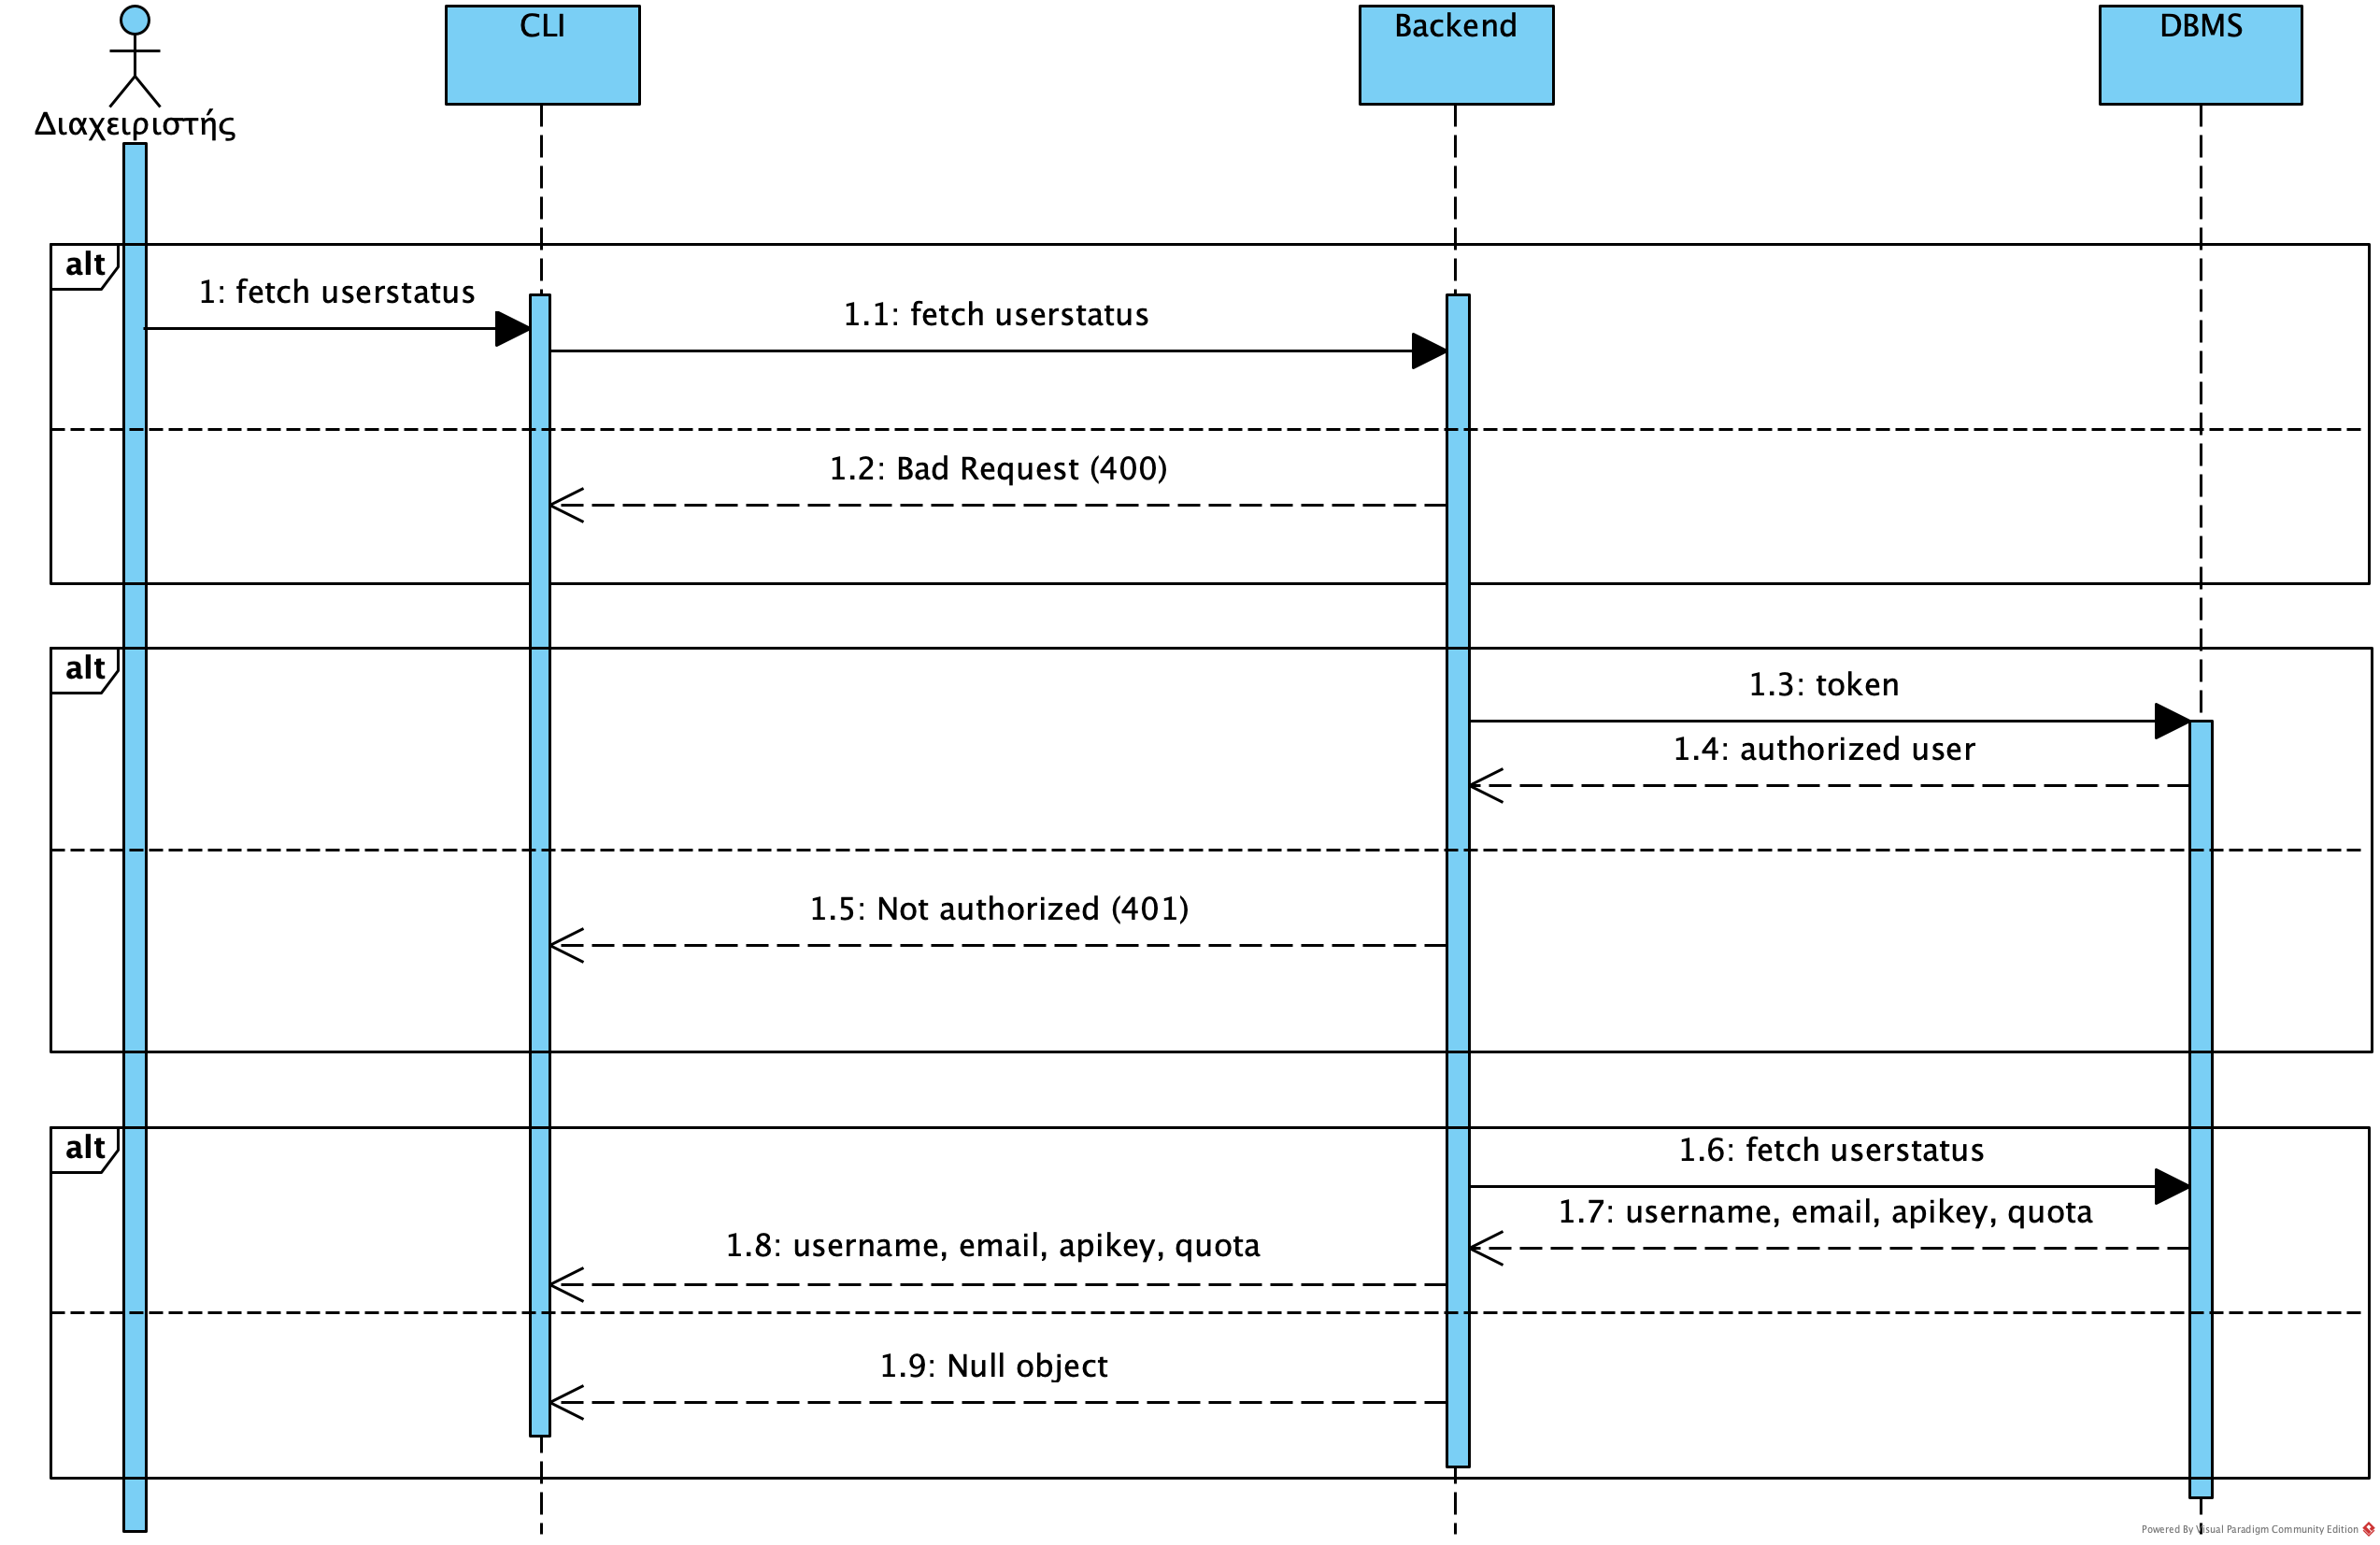
\includegraphics[width=1\textwidth]{./UML/Sequence_Diagram_Admin_fetch_userstatus.png}
\caption{\textlatin{Sequence diagram} ανάκτησης πληροφοριών για κάποιο χρήστη από τον Διαχειριστή}
\centering
\end{figure}



\newpage
\subsection{Απαιτήσεις επιδόσεων}
Έχοντας κατά νου ότι το λογισμικό μας θα είναι συνεχώς διαθέσιμο στους χρήστες και πως σε μια εφαρμογή πραγματικού κόσμου σχεδόν όλα τα αιτήματα αλληλεπιδρούν με τη βάση δεδομένων, υλοποιήσαμε την πλατφόρμα χρησιμοποιώντας \textlatin{Node.js} με \textlatin{Express JS} που έχουν πολύ υψηλή απόδοση ακόμα για πολλά αιτήματα ανά δευτερόλεπτο. Ενδεικτικά, ένας διακομιστής με καλή σχέση κόστους-απόδοσης θα ήταν με 4 πυρήνες και 8 \textlatin{GB} μνήμη\footnote{\textlatin{\href{https://medium.com/@mihaigeorge.c/web-rest-api-benchmark-on-a-real-life-application-ebb743a5d7a3}{https://medium.com/@mihaigeorge.c/web-rest-api-benchmark-on-a-real-life-application-ebb743a5d7a3}}}.

Ακολουθούν οι μετρικές που γενικά μας ενδιαφέρουν για την αξιολόγηση του \textlatin{back-end}.
\begin{itemize}
	\item \textbf{\textlatin{Throughput}}: υποδεικνύει τον όγκο της κυκλοφορίας που διαχειρίζεται μια υπηρεσία. Γενικά υπό υψηλή πίεση, ένας διακομιστής είναι γενικά βραδύτερος από αυτόν σε κανονικό φορτίο.
	\item \textbf{\textlatin{Latency}}: υποδεικνύει το χρόνο ολοκλήρωσης μίας λειτουργίας I/O. Στην περίπτωσή μας, αναμένουν ανατροφοδότηση σε πραγματικό χρόνο μετά από κάθε είσοδο ενός χαρακτήρα. Σχετίζεται με το \textlatin{throughput}, δηλαδή η αύξηση του \textlatin{throughput} συνοδεύεται από παράλληλη αύξηση του \textlatin{latency}.
	\item \textbf{\textlatin{Error rate}}: τα \textlatin{error} που δημιουργούνται από ζητήματα δικτύου (π.χ. συμφόρηση)  δεν πρέπει να υπερβαίνουν το 5\% των συνολικών αιτημάτων και τα \textlatin{error}  που προκλήθηκαν από την εφαρμογή δεν πρέπει να υπερβαίνουν το 1\%.
\end{itemize} 


\subsection{Απαιτήσεις οργάνωσης δεδομένων}
\subsubsection{Απαιτήσεις και περιορισμοί πρόσβασης σε δεδομένα}
Υπάρχουν δύο διαφορετικές κατηγορίες χρηστών, εκάστη με τις δικές της απαιτήσεις και περιορισμούς πρόσβασης.
\begin{itemize}
    \item \textbf{Απλός Χρήστης}: Ο Απλός Χρήστης έχει πρόσβαση στα δεδομένα παραγωγής, κατανάλωσης, εκτιμώμενης κατανάλωσης και στις συγκρίσεις τους.  Όμως η πρόσβαση του στα δεδομένα περιορίζεται σε συγκεκριμένο πλήθος κλήσεων της εφαρμογής ανά ημέρα \textlatin{(quota)}.  
    \item \textbf{Διαχειριστής}: Ο Διαχειριστής έχει τη δυνατότητα να παρακολουθεί και να διαμορφώνει όλα τα δεδομένα στη βάσης δεδομένων, είτε πρόκειτε για εγγραφές ενέργειας είτε χρηστών. 
\end{itemize}


\newpage
\subsection{Περιορισμοί σχεδίασης}
Αρχικά αναφέρουμε τα  εργαλεία που χρησιμοποιήσαμε για την υλοποίηση της πλατφόρμας.
\begin{itemize}
    \item \textbf{\textlatin{MySQL}} για τη σχεσιακή βάση δεδομένων
    \item \textbf{\textlatin{JavaScript}}
    \item \textbf{\textlatin{Node.js}} \textlatin{framework} της \textlatin{JavaScript}
    \item \textbf{\textlatin{Express}} \textlatin{framework} για το \textlatin{Node.js}
    \item \textbf{\textlatin{npm}} για το \textlatin{build automation} 
    \item \textbf{\textlatin{SSH}} για πρόσβαση στον server
\end{itemize}


\subsection{Λοιπές απαιτήσεις}
\subsubsection{Απαιτήσεις διαθεσιμότητας λογισμικού}
Οι απλοί χρήστες, που είναι εγγεγραμμένοι, έχουν δυνατότητες προσπέλασης δεδομένων και ελέγχου της  συνδεσιμότητας \textlatin{(end-to-end connectivity)} τους με τη βάση δεδομένων \textlatin{(HealthCheck)}. Ο διαχειριστής του συστήματος έχει δυνατότητες δημιουργίας και επεξεργασίας χρήστη, εμφάνισης κατάστασης δοσμένου χρήστη, προσθήκης νέων δεδομένων στη βάση από έγγραφο \textlatin{.csv}, «εκκαθάρισης» της βάσης από κάθε δεδομένο πέραν του διαχειριστικού λογαριασμού \textlatin{(reset)} και ελέγχου της  συνδεσιμότητας \textlatin{(end-to-end connectivity)} του με τη βάση δεδομένων \textlatin{(HealthCheck)}.   

\subsubsection{Απαιτήσεις ασφάλειας}
Το σύστημα υποστηρίζει το πρωτόκολλο \textlatin{HTTPS} για όλες τις χρηστικές και προγραμματιστικές διεπαφές μέσω \textlatin{self-signed certificate}, για να διασφαλίσει ότι τα προσωπικά δεδομένα των χρηστών είναι απροσπέλαστα. Χρησιμοποιεί επίσης ένα επιπλέον επίπεδο ασφαλείας,  με \textlatin{hash authentication}, για τους κωδικούς πρόσβασης των χρηστών. Τέλος, αν και τα δεδομένα που επιστρέφονται από τα \textlatin{endpoints} ανάκτησης και αναζήτησης δεδομένων του \textlatin{API}  προσφέρονται ως ανοικτά δεδομένα \textlatin{(Open Data)}, για λόγους ελέγχου της κατανάλωσης πόρων του συστήματος που τα διαθέτει, για τη χρήση του \textlatin{API} θα απαιτείται διαπίστευση των χρηστών. Συνεπώς, κατά την κλήση του \textlatin{API} παρέχεται το \textlatin{user access token}, κωδικοποιημένο μέσα σε \textlatin{custom HTTP Header}, το όνομα του οποίου είναι \textlatin{XOBSERVATORY-AUTH.}

\subsubsection{Απαιτήσεις συντήρησης}
Πρέπει ανά τακτά διαστήματα να ενημερώνεται το λογισμικό και η βάση δεδομένων, ώστε το σύστημα να παραμένει συμβατό με τις νέες εκδόσεις των γλωσσών και των τεχνολογικών εργαλείων που χρησιμοποιεί. Ακόμη, απαιτείται η ύπαρξη ενός εφεδρικού διακομιστή ώστε η πλατφόρμα να είναι διαρκώς διαθέσιμη, ακόμα και όταν ο \textlatin{server}  χρήζει συντήρησης.


\newpage
\section{Παράρτημα: ακρωνύμια και συντομογραφίες}
\textlatin{\textbf{API} Application Programming Interface\\
\textbf{REST API} RESTful Application Programming Interface\\
\textbf{CLI} Command Line Interface\\
\textbf{JSON} JavaScript Object Notation\\
\textbf{HTTP} Hypertext Transfer Protocol\\
\textbf{HTTPS} Hypertext Transfer Protocol Secure\\
\textbf{SSH} Secure Shell \\
\textbf{SQL}  Structured Query Language\\
\textbf{JS} JavaScript\\
\textbf{npm} Node Package Manager\\
\textbf{UML} Unified Modeling Language\\
\textbf{SRS} Software Requirements Specification 
}
\end{document}  